\tikzset{every picture/.style={line width=0.75pt}} %set default line width to 0.75pt        

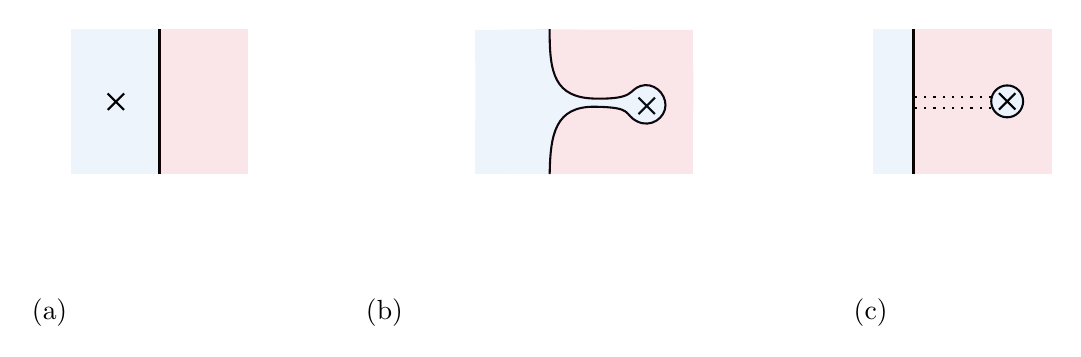
\begin{tikzpicture}[x=0.75pt,y=0.75pt,yscale=-1,xscale=1]
%uncomment if require: \path (0,300); %set diagram left start at 0, and has height of 300

%Shape: Rectangle [id:dp23227140038029304] 
\draw  [draw opacity=0][fill={rgb, 255:red, 74; green, 144; blue, 226 }  ,fill opacity=0.1 ] (61.17,86.85) -- (104,86.85) -- (104,156.85) -- (61.17,156.85) -- cycle ;
%Straight Lines [id:da24044805644262146] 
\draw    (104,87) -- (104,156.85) ;
%Straight Lines [id:da6746174603382504] 
\draw    (83,122) ;
\draw [shift={(83,122)}, rotate = 45] [color={rgb, 255:red, 0; green, 0; blue, 0 }  ][line width=0.75]    (-5.59,0) -- (5.59,0)(0,5.59) -- (0,-5.59)   ;
%Straight Lines [id:da8992839725832915] 
\draw    (338.75,124) ;
\draw [shift={(338.75,124)}, rotate = 45] [color={rgb, 255:red, 0; green, 0; blue, 0 }  ][line width=0.75]    (-5.59,0) -- (5.59,0)(0,5.59) -- (0,-5.59)   ;
%Curve Lines [id:da20801752082073] 
\draw    (292,87) .. controls (291.79,108.44) and (294.37,120.1) .. (313.83,120.52) .. controls (333.29,120.94) and (329.79,116.44) .. (335.79,114.44) .. controls (341.79,112.44) and (347.79,117.69) .. (347.79,123.69) .. controls (347.79,129.69) and (340.79,134.94) .. (334.04,131.44) .. controls (327.29,127.94) and (332.79,124.69) .. (313.79,124.44) .. controls (294.79,124.19) and (292.29,137.44) .. (292,156.85) ;
%Shape: Rectangle [id:dp17248129737182882] 
\draw  [draw opacity=0][fill={rgb, 255:red, 208; green, 2; blue, 27 }  ,fill opacity=0.1 ] (104,86.85) -- (146.83,86.85) -- (146.83,156.85) -- (104,156.85) -- cycle ;
%Curve Lines [id:da39495239856656794] 
\draw [draw opacity=0][fill={rgb, 255:red, 74; green, 144; blue, 226 }  ,fill opacity=0.1 ]   (292,87) .. controls (291.79,108.44) and (294.37,120.1) .. (313.83,120.52) .. controls (333.29,120.94) and (329.79,116.44) .. (335.79,114.44) .. controls (341.79,112.44) and (347.79,117.69) .. (347.79,123.69) .. controls (347.79,129.69) and (340.79,134.94) .. (334.04,131.44) .. controls (327.29,127.94) and (332.79,124.69) .. (313.79,124.44) .. controls (294.79,124.19) and (292.29,137.44) .. (292,156.85) .. controls (280.54,157.02) and (278.54,156.77) .. (256,156.85) .. controls (256.29,94.1) and (256.33,136.46) .. (256.04,87.35) .. controls (276.04,87.6) and (258.29,87.1) .. (292,87) -- cycle ;
%Curve Lines [id:da6144255835160188] 
\draw [draw opacity=0][fill={rgb, 255:red, 208; green, 2; blue, 27 }  ,fill opacity=0.1 ]   (292,87) .. controls (291.79,108.44) and (294.37,120.1) .. (313.83,120.52) .. controls (333.29,120.94) and (329.79,116.44) .. (335.79,114.44) .. controls (341.79,112.44) and (347.79,117.69) .. (347.79,123.69) .. controls (347.79,129.69) and (340.79,134.94) .. (334.04,131.44) .. controls (327.29,127.94) and (332.79,124.69) .. (313.79,124.44) .. controls (294.79,124.19) and (292.29,137.44) .. (292,156.85) .. controls (280.54,157.02) and (383.54,156.77) .. (361,156.85) .. controls (361.29,94.1) and (361.33,136.46) .. (361.04,87.35) .. controls (381.04,87.6) and (258.29,87.1) .. (292,87) -- cycle ;
%Shape: Rectangle [id:dp7140929144714487] 
\draw  [draw opacity=0][fill={rgb, 255:red, 74; green, 144; blue, 226 }  ,fill opacity=0.1 ] (447.61,87) -- (467.28,87) -- (467.28,157) -- (447.61,157) -- cycle ;
%Straight Lines [id:da4713286386748359] 
\draw    (467.28,87) -- (467.28,156.85) ;
%Shape: Rectangle [id:dp9307193592961596] 
\draw  [draw opacity=0][fill={rgb, 255:red, 208; green, 2; blue, 27 }  ,fill opacity=0.1 ] (467.28,86.85) -- (533.83,86.85) -- (533.83,156.85) -- (467.28,156.85) -- cycle ;
%Shape: Circle [id:dp020567399671055364] 
\draw  [fill={rgb, 255:red, 255; green, 255; blue, 255 }  ,fill opacity=1 ] (504.74,121.85) .. controls (504.74,117.62) and (508.18,114.18) .. (512.42,114.18) .. controls (516.65,114.18) and (520.09,117.62) .. (520.09,121.85) .. controls (520.09,126.09) and (516.65,129.53) .. (512.42,129.53) .. controls (508.18,129.53) and (504.74,126.09) .. (504.74,121.85) -- cycle ;
%Shape: Circle [id:dp18933498134489657] 
\draw  [draw opacity=0][fill={rgb, 255:red, 74; green, 144; blue, 226 }  ,fill opacity=0.1 ] (504.74,121.85) .. controls (504.74,117.62) and (508.18,114.18) .. (512.42,114.18) .. controls (516.65,114.18) and (520.09,117.62) .. (520.09,121.85) .. controls (520.09,126.09) and (516.65,129.53) .. (512.42,129.53) .. controls (508.18,129.53) and (504.74,126.09) .. (504.74,121.85) -- cycle ;
%Straight Lines [id:da2894948145731697] 
\draw    (512.42,121.85) ;
\draw [shift={(512.42,121.85)}, rotate = 45] [color={rgb, 255:red, 0; green, 0; blue, 0 }  ][line width=0.75]    (-5.59,0) -- (5.59,0)(0,5.59) -- (0,-5.59)   ;
%Straight Lines [id:da05776141758085607] 
\draw  [dash pattern={on 0.84pt off 2.51pt}]  (504.74,119.85) -- (467.28,119.85) ;
%Straight Lines [id:da9078103279098249] 
\draw  [dash pattern={on 0.84pt off 2.51pt}]  (504.74,124.85) -- (467.28,124.85) ;

% Text Node
\draw (41,215.5) node [anchor=north west][inner sep=0.75pt]   [align=left] {(a)};
% Text Node
\draw (202,215.5) node [anchor=north west][inner sep=0.75pt]   [align=left] {(b)};
% Text Node
\draw (437,215.5) node [anchor=north west][inner sep=0.75pt]   [align=left] {(c)};


\end{tikzpicture}
